\section{Разработка системы вычисления и передачи данных о положении дрона}

Отправка видеопотока производится посредством UDP протокола. Его выбор обоснован спецификой передаваемых данных: видеотрансляция в режиме реального времени, и чтобы не выполнять пересыл отправленных пакетов, вместо TCP решено использовать UDP.
% дописано
Так как системе критична задержка видеосигнала, необходимо использовать кодек. Кодек -- программный алгоритм сжатия видео, но он настолько часто используется в современных системах, что его поддержку реализуют на аппаратном уровне во многих современных процессорах. Из доступных кодеков можно выделить jpeg, h264, omxh264enc. Первые два являются программными, третий -- аппаратный.
В нашей системе есть аппаратная реализация кодека h264. Но, к сожалению, пока не получилось добиться его стабильной работы, частично это связано с архитектурными особенностями и закрытостью видеоподсистемы RPi \cite{rpi}. Стабильнее всего проявил себя кодек h264. Задержка составила 150 мс.

После включения дрона и загрузки ОС RPi производится удаленное подключение к Raspberry Pi.
Запускается gstreamer для передачи изображения с rpicamsrc на адрес наземной станции UDP пакетами. gst-launch оказался очень трепетным к pipeline, в ходе выполнения НИР ушло довольно много времени на подбор параметров для трансляции. Итоговая команда представлена в листинге \ref{lst:12}:
\begin{Program}[H]
	\caption{Команда запуска gstreamer} \label{lst:12}
\begin{MyCode}
$ gst-launch-1.0 rpicamsrc bitrate=1000000 !\
'video/x-h264,width=640,height=480' ! h264parse !\
queue ! rtph264pay config-interval=1 pt=96 ! gdppay !\
udpsink host=[IP ПК] port=5000
\end{MyCode}
\end{Program}

На наземной станции в первой вкладке консоли запускается окружение mavros (листинг\ref{lst:13} ):
\begin{Program}[H]
\caption{Команда запуска окружения mavros} \label{lst:13}
\begin{MyCode}
$ roslaunch mavros px4.launch
\end{MyCode}
\end{Program}

После того, как произошли подключение и инициализация дрона в окружении, во второй вкладке консоли производится сброс координат дрона (инициализация параметров SET\_GPS\_GLOBAL\_ORIGIN и SET\_HOME\_POSITION) (листинг \ref{lst:14}):
\begin{Program}[H]
	\caption{Команда сброса координат дрона} \label{lst:14}
\begin{MyCode}
$ rosrun aruco_gridboard set_origin.py
\end{MyCode}
\end{Program}

В третьей вкладке консоли запускается aruco\_gridboard, совмещенный с нодой gscam, для получения и обработки изображения (листинг \ref{lst:15}):
\begin{Program}[H]
\caption{Команды запуска aruco\_gridboard с нодой gscam} \label{lst:15}
\begin{MyCode}
$ export GSCAM_CONFIG="udpsrc port=5000 ! gdpdepay !\
rtph264depay ! avdec_h264 ! videoconvert"
$ roslaunch aruco_gridboard detection_rpicam.launch 
\end{MyCode}
\end{Program}

На рисунке \ref{fig:ar} представлена схема взаимодействия в этот момент дрона и наземной станции.

\begin{figure}[H]
\centering
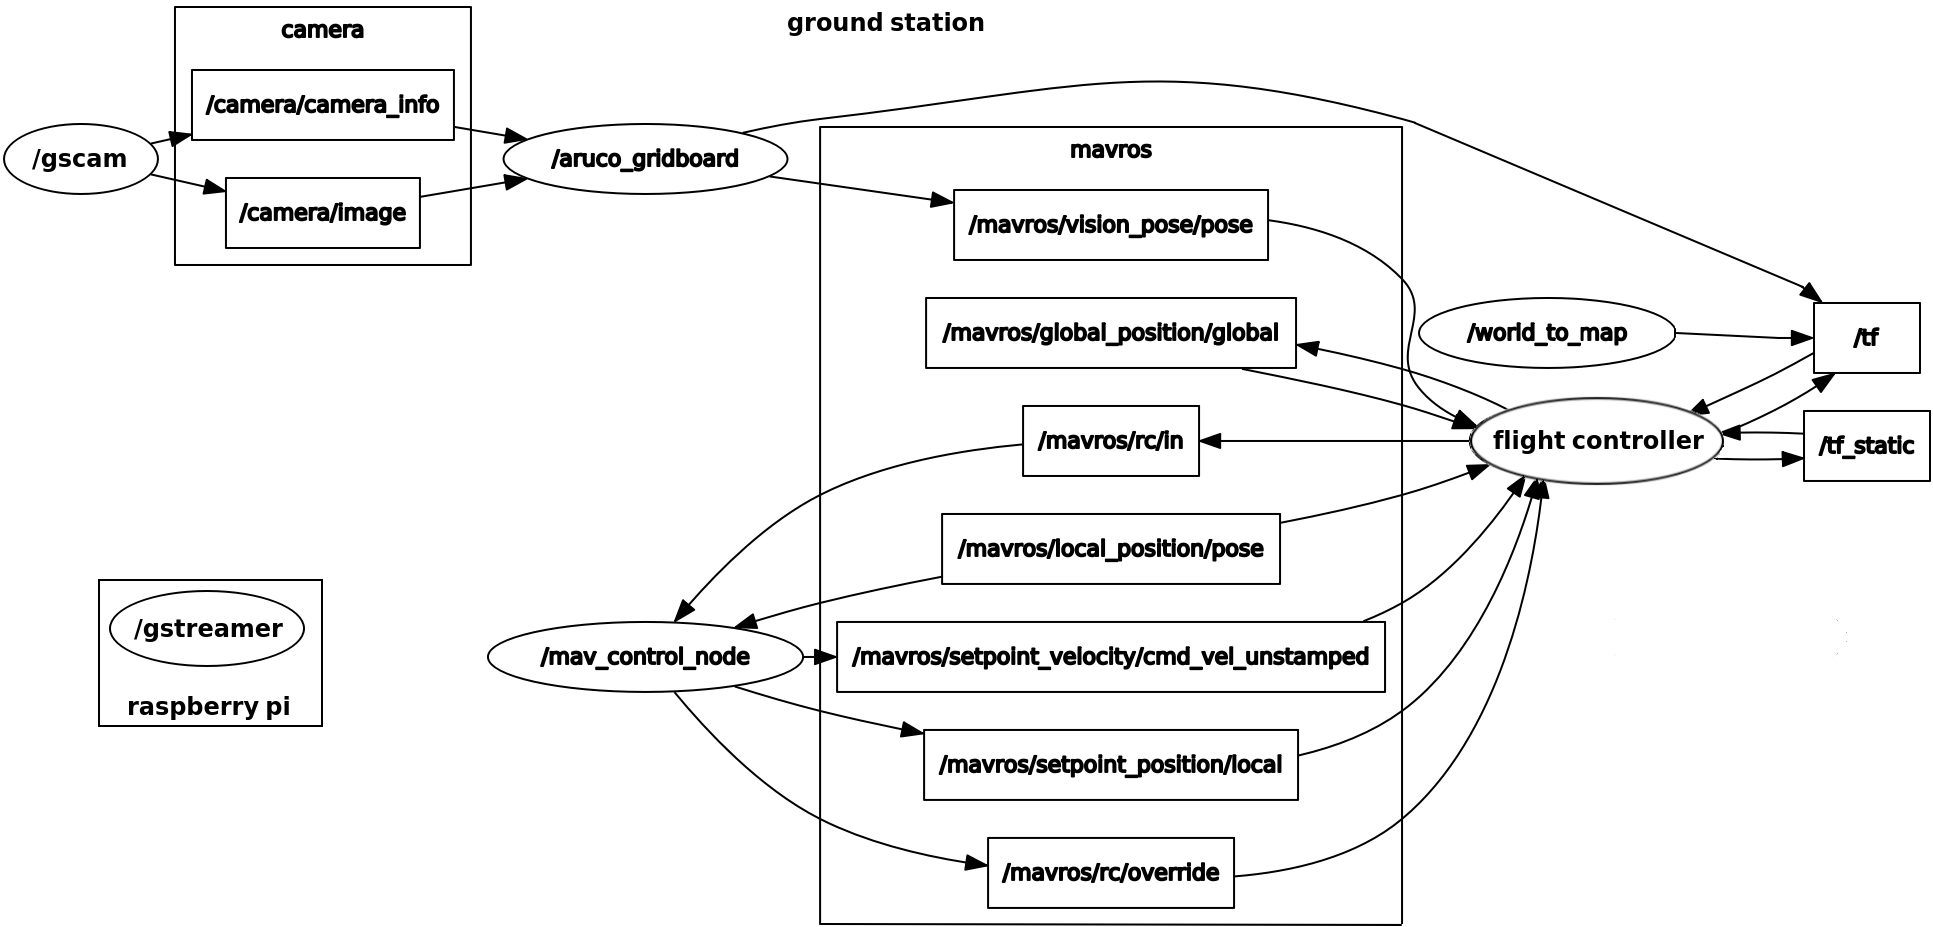
\includegraphics[width=0.95\linewidth]{./pics/graph}
\caption{Архитектура спроектированной системы
}
\label{fig:ar} % эта метка позволяет ссылаться на рисунок в тексте
\end{figure}

Для проверки корректности работы системы можно запустить программу rviz -- инструмент 3D-визуализации для ROS (листинг \ref{lst:16}):
\begin{Program}[H]
\caption{Команда запуска rviz} \label{lst:16}
\begin{MyCode}
$ rosrun rviz rviz -d catkin_ws/src/aruco_gridboard/data/aruco_grid.rviz
\end{MyCode}
\end{Program}

На рисунке \ref{fig:px4} отображены: вывод в консоль координат, полученных aru\-co\_g\-rid\-board, изображение с камеры дрона с началом координат на карте маркеров и поле rviz с моделью дрона относительно карты.
% ~\ref{fig:px4}
\begin{figure}[H]
	\centering
	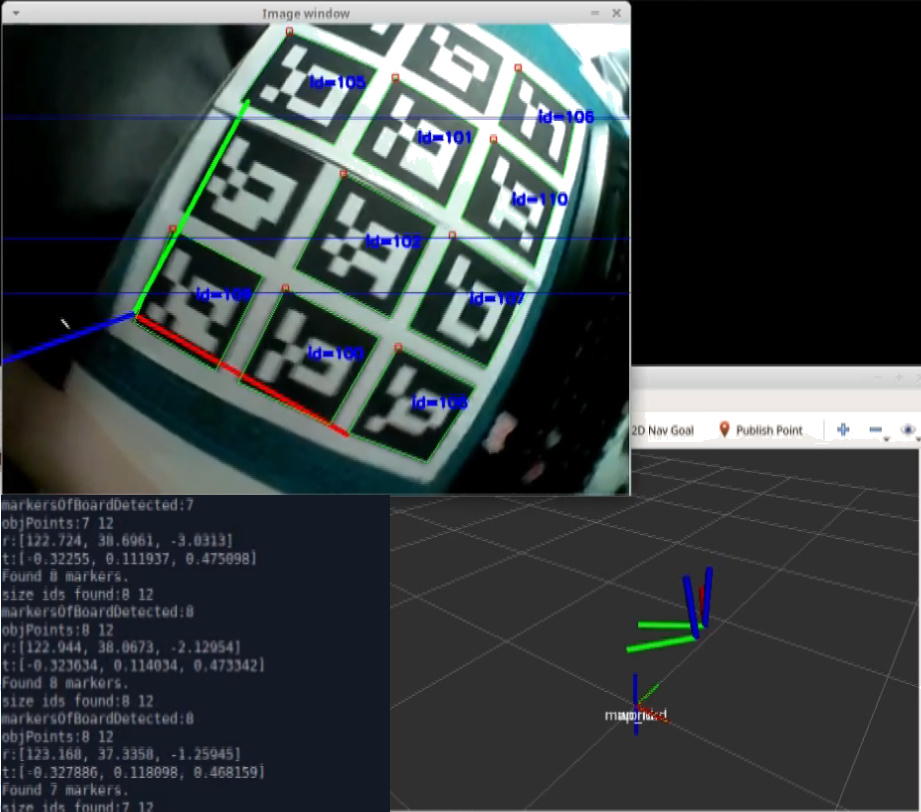
\includegraphics[width=0.7\linewidth]{pics/px4}
	\caption{ Скриншот экрана наземной станции во время определения положения дрона
	}
	\label{fig:px4}
\end{figure}

Система готова к использованию. С помощью команды, представленной в листинге \ref{lst:17}, запускается автономная миссия (код mavros\_control.py находится в приложении А):
\begin{Program}[H]
\caption{Команда запуска автономной миссии} \label{lst:17}
\begin{MyCode}
$ rosrun aruco_gridboard mavros_control.py
\end{MyCode}
\end{Program}
